\subsection{Browserunterstützung der \acs{pwa}}
Für Webanwendungen ist es üblich, diese mit verschiedenen Browsern zu testen. Um das Kriterium der Plattformabhängigkeit detailliert evaluieren zu können, erscheint es ebenfalls sinnvoll, die Installation der PWA sowohl auf dem Desktop, als auch auf Android und iOS Smartphones zu testen.

\textbf{Anmerkung:}\\
Zum Testen der Datenpersistenz werden Todo-Einträge angelegt und anschließend der Browser neugestartet.
Alle Browser werden mit Standardeinstellungen ausgeführt. Es werden keine Browsercaches, Cookies oder ähnliches manuell gelöscht.

\textbf{Desktop:}

\begin{table}[H]
	\centering
	\begin{tabularx}{\textwidth}{|l||C|C|C|C|}
		\hline
		Browser              & Anwendung lauffähig & Persistente Daten & PWA installierbar & Benachrichtigungen \\
		\hline
		Chrome 78 (64-bit)   & Ja                  & Ja                & Ja                & Ja                 \\
		Firefox 70 (64-bit)  & Ja                  & Ja                & Nein              & Ja                 \\
		Microsoft Edge 41    & Ja                  & Ja                & Nein              & Nein               \\
		Internet Explorer 11 & Ja                  & Ja                & Nein              & Nein               \\
		Safari 13            & Ja                  & Ja                & Nein              & Nein               \\
		\hline
	\end{tabularx}
	\caption{Browserunterstützung Desktop} \label{tab:browser_desktop}
\end{table}

\textbf{Anmerkung:}\\
Microsoft Edge und Internet Explorer zeigen den Button zum Priorisieren nicht an. Dieser enthält ein Unicodezeichen eines Sterns.

Microsoft Edge möchte die Zustimmung des Nutzers, um Benachrichtigungen anzuzeigen, zeigt jedoch anschließend keine Benachrichtigungen an. Internet Explorer wirft den JavaScript Fehler \texttt{'Notification' is undefined}, Notifications sind nicht implementiert.

\textbf{Smartphone:}

\begin{table}[H]
	\centering
	\begin{tabularx}{\textwidth}{|l||C|C|C|C|}
		\hline
		Browser           & Anwendung lauffähig & Persistenz & PWA installierbar & Benachrichtigungen \\
		\hline
		\multicolumn{5}{|c|}{Android}                                                                 \\
		\hline
		Chrome 78         & Ja                  & Ja         & Ja                & Ja                 \\
		Firefox 68        & Ja                  & Ja         & Ja                & Ja                 \\
		Microsoft Edge 41 & Ja                  & Ja         & Nein              & Ja                 \\
		Opera 54          & Ja                  & Ja         & Nein              & Ja                 \\
		\hline
		\multicolumn{5}{|c|}{iOS}                                                                     \\
		\hline
		Chrome            & Ja                  & Ja         & Nein              & Nein               \\
		Safari 13         & Ja                  & Ja         & Nein              & Nein               \\
		\hline
	\end{tabularx}
	\caption{Browserunterstützung Smartphones} \label{tab:browser_smartphones}
\end{table}

\textbf{Anmerkung:}\\
Verweigert der Nutzer die Benachrichtigungen einer Webseite, ist es meist umständlich die Berechtigung für Benachrichtigungen einer Website zurückzusetzen. Beim Browser Opera muss der Nutzer dann beispielsweise durch fünf Menüs nacheinander navigieren, um die deaktivierten Benachrichtigungen wieder zu aktivieren.


%	Plattformabhängikeit   & 0   & 1 & 2       & 3 & 4  & 10\%         \\
%Installation           & 0   & 1 & 2       & 3 & 4  & 5\%          \\
%Speicherzugriff        & 0   & 1 & 2       & 3 & 4  & 5\%          \\
%Speicherbedarf         & 0   & 1 & 2       & 3 & 4  & 5\%          \\
%Aktualisierbarkeit     & 0   & 1 & 2       & 3 & 4  & 5\%          \\
%Konsistenz des Designs & 0   & 1 & 2       & 3 & 4  & 5\%         \\
%Bibliotheken           & 0   & 1 & 2       & 3 & 4  & 10\%         \\
%Umsetzung              & 0   & 1 & 2       & 3 & 4  & 20\%         \\
%Testbarkeit            & 0   & 1 & 2       & 3 & 4  & 10\%         \\
%Vorausgesetzte Entwicklungserfahrung    & 0   & 1 & 2       & 3 & 4  & 10\%         \\
%Verständlichkeit       & 0   & 1 & 2       & 3 & 4  & 10\%         \\
%
\begin{figure}[h]

	\begin{tikzpicture}
	
		% Diagram setup
		\tkzKiviatDiagram[scale=1.0,label distance=.5cm,
		radial  = 4,
		gap     = 1,  
		lattice = 4]{
			Plattformabhängigkeit,
			Installation,
			Speicherzugriff,
			Speicherbedarf,
			Aktualisierbarkeit,
			Designs,
			Bibliotheken,
			Umsetzung,
			Testbarkeit,
			Vorausgesetzte Entwicklungserfahrung,
			Nutzerfreundlichkeit
		}
		
		% native App
		\tkzKiviatLine[thick,color=blue,mark=ball,
		fill=blue!20,opacity=.5](2,4,4,2,3,3,1,2,3,3,4)
		
		% PWA
		\tkzKiviatLine[thick,color=green,mark=ball,
		fill=green!20,opacity=.5](3,2,3,4,4,1,4,4,4,1,2)
		
		\tkzKiviatGrad[prefix=,unity=1,suffix=](0)  
	

	
	\end{tikzpicture}
	
	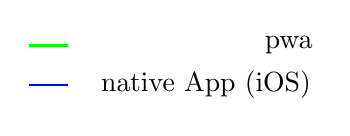
\begin{tikzpicture}
	%\draw[draw=black!20] (-0.1,-0.2) rectangle ++(15,0.5);
	
	\draw [thick, green] (0,0.5) -- (0.5,0.5); 
	\node at (3.3,0.5) {\acf{pwa}};
	
	\draw [thick, blue] (0,0) -- (0.5,0); 
	\node at (2.25,0) {native App (iOS)};
	

		\end{tikzpicture}
	
	\caption{Spinnennetzdiagram: Kriterienvergleich \acs{pwa} und native App}
\end{figure}